\documentclass[11pt,a4paper,oneside]{article}
\usepackage{geometry}
\usepackage[pdftex]{graphicx}
\usepackage{graphicx}
\usepackage{sidecap}
\usepackage{amsmath}

\newenvironment{amatrix}[1]{%
  \left[\begin{array}{@{}*{#1}{c}|c@{}}
}{%
  \end{array}\right]
}

\begin{document}

\title{ISC5907 - Prelim Preparation Class \\ 
	 Summer 2015 Prelim Exam Question 10}
\author{Stephen Alexander Townsend}
\date{\today}
\maketitle

\section{Question 10: Monte-Carlo Integration}
%##################################################
\subsection{Question 1a: Numerical Integral and Error}
   The function evaluations and the error estimates are computed by a MATLAB program which was
submitted along with the answers to this question.  

\subsection{Question 1b: Analytical Variance and Comparison}
   Here, I derive the analytical error variance for the given equation and compare to the 
numerically computed error variance.

\begin{equation}
	\sigma^2_I = \frac{<f^2> - <f>^2}{n}
\end{equation}

Because we are told that $<f> = I(\gamma)$ and that $<f^2> = \int_0^1 x^{2\gamma} dx$, we
can compute the analytical variance $<f^2> - <f>^2$.  Which is the same as the error variance
above but without the $n$ indicating number of samples.

\begin{equation}
	<f> = I(\gamma) = \int_0^1 x^{\gamma} dx = \frac{1}{\gamma + 1}
\end{equation}
\begin{equation}
	<f^2> = I(2\gamma) = \int_0^1 x^{2\gamma} dx = \frac{1}{2\gamma + 1}
\end{equation}
\begin{equation}
	<f>^2 = \big(\frac{1}{\gamma + 1})^2 = \frac{1}{(\gamma + 1)^2}
\end{equation}
\begin{equation}
	<f^2> - <f>^2 = \frac{1}{2\gamma + 1} - \frac{1}{(\gamma + 1)^2}
\end{equation}

For the two given values of $\gamma$, $-0.2$ and $-0.9$, this analytical expression becomes:

\begin{equation}
	\big( <f^2> - <f>^2\big) \big|_{-0.2} = 0.10417
\end{equation}
\begin{equation}
	\big( <f^2> - <f>^2\big) \big|_{-0.9} = -101.25
\end{equation}

From the above derivation, it is obvious that we would expect a very large variance in the error
as $\gamma \rightarrow -1$.  Shown below is a graph of the numerical vs. expected standard deviation
in the error, which is simply the square root of equation (1) given above.  As you can see, we get
exactly what was expected from the analytical results above.

\begin{centering}
\begin{figure}[h!]
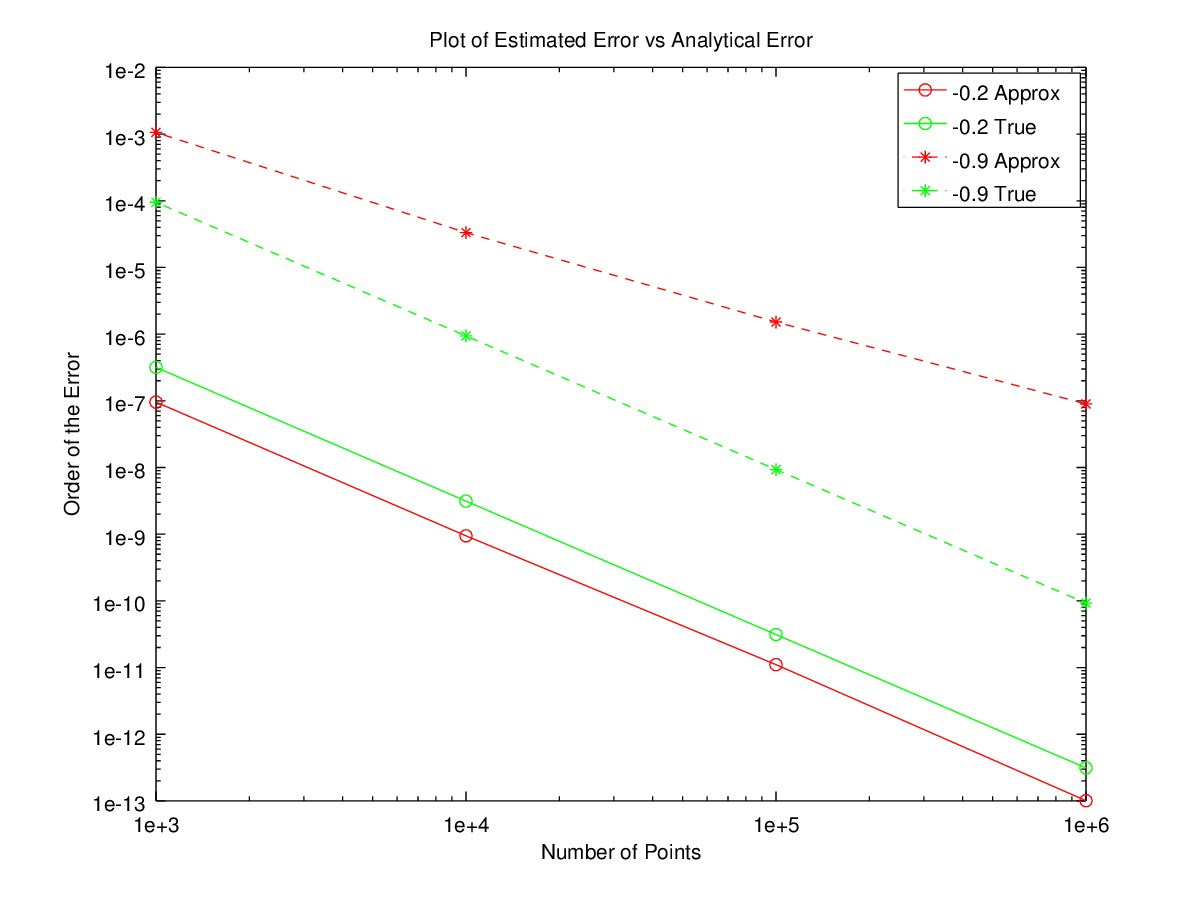
\includegraphics[width=\textwidth]{untitled.png}
\caption{Comparison of analytical error (solid lines) vs. numerical error (dashed lines).}
\end{figure}
\end{centering}

\end{document}
